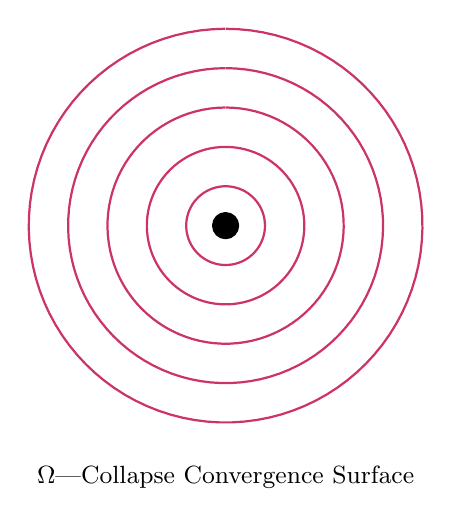
\begin{tikzpicture}[
    event/.style={circle, fill=white, draw=black, minimum size=6pt, thick},
    collapse/.style={circle, fill=black, draw=black, minimum size=7pt},
    spiral/.style={thick, draw=purple!80}
]

\foreach \r in {0.5,1,1.5,2,2.5}{
    \draw[spiral] (0,0) plot [domain=0:6.28,samples=100]
       ({\r*sin(\x r)}, {\r*cos(\x r)});
}

\node[collapse] at (0,0) {};
\node at (0,-3.2) {\small $\Omega$---Collapse Convergence Surface};

\end{tikzpicture}